% !TeX root = ./eLife_draft.tex

%%%%%%%%%%%%%%%%%%%%%%%%%%%%%%%%%%%%%%%%%%%%%%%%%%%%%%%%%%%%
%%% ELIFE ARTICLE TEMPLATE
%%%%%%%%%%%%%%%%%%%%%%%%%%%%%%%%%%%%%%%%%%%%%%%%%%%%%%%%%%%%
%%% PREAMBLE
\documentclass[9pt,lineno]{elife}
% Use the onehalfspacing option for 1.5 line spacing
% Use the doublespacing option for 2.0 line spacing
% Please note that these options may affect formatting.
% Additionally, the use of the \newcommand function should be limited.

\usepackage{lipsum} % Required to insert dummy text
\usepackage[version=4]{mhchem}
\usepackage{siunitx}
\DeclareSIUnit\Molar{M}

%%%%%%%%%%%%%%%%%%%%%%%%%%%%%%%%%%%%%%%%%%%%%%%%%%%%%%%%%%%%
%%% ARTICLE SETUP
%%%%%%%%%%%%%%%%%%%%%%%%%%%%%%%%%%%%%%%%%%%%%%%%%%%%%%%%%%%%

\title{Fundamental limits on the rate of bacterial cell division}
\author[$\dagger$, 1]{Nathan M. Belliveau}
\author[$\dagger$, 2, 3]{Griffin Chure}
\author[4]{Christina L. Hueschen}
\author[5]{Hernan G. Garcia}
\author[6]{Jan\'{e} Kondev}
\author[7]{Daniel S. Fisher}
\author[1, 8]{Julie Theriot}
\author[1, 2, 9, *]{Rob Phillips}
\affil[1]{Department of Biology, University of Washington, Seattle, WA, USA}
\affil[2]{Division of Biology and Biological Engineering, California Institute of Technology, Pasadena, CA, USA}
\affil[3]{Department of Applied Physics, California Institute of Technology, Pasadena, CA, USA}
\affil[4]{Department of Chemical Engineering, Stanford University, Stanford, CA, USA}
\affil[5]{Department of Molecular Cell Biology and Department of Physics, University of California Berkeley, Berkeley, CA, USA}
\affil[6]{Department of Physics, Brandeis University, Waltham, MA, USA}
\affil[7]{Department of Applied Physics, Stanford University, Stanford, CA, USA}
\affil[8]{Allen Institute for Cell Science, Seattle, WA, USA}
\affil[9]{Department of Physics, California Institute of Technology, Pasadena, CA, USA}
\affil[*]{Contributed equally}
\contrib[$\dagger$]{These authors contributed equally to this work}

%%%%%%%%%%%%%%%%%%%%%%%%%%%%%%%%%%%%%%%%%%%%%%%%%%%%%%%%%%%%
%%% ARTICLE START
%%%%%%%%%%%%%%%%%%%%%%%%%%%%%%%%%%%%%%%%%%%%%%%%%%%%%%%%%%%%

\begin{document}

\maketitle

\begin{abstract}

\end{abstract}

% % !TeX root = ./eLife_draft.tex

\section{Introduction}
The observed range of bacterial growth rates is enormously diverse. In natural
environments, some microbial organisms may double only once per year
\citep{mikucki2009} while in comfortable laboratory conditions, growth can be
rapid with several divisions per hour \citep{schaechter1958}. This six
order-of-magnitude difference in time scales of growth encompasses different
microbial species and lifestyles, yet even for a single species such as
\textit{Escherichia coli}, the growth rate can be modulated over a
large scale by tuning the type and amount of nutrients in the growth medium
\citep{liu2005a}. This remarkable plasticity in growth rate illustrates the
intimate relationship between environmental conditions and the rates at which
cells convert nutrients into new cellular material -- a relationship that has
remained a major topic of inquiry in bacterial physiology for over a century
\citep{jun2018}.

A key discovery in bacterial physiology of the past 70 years was the
identification of bacterial "growth laws" \citep{schaechter1958}; empirical
relationships that relate the bacterial growth rate to the protein and RNA
composition of the intracellular milieu in a number of different species.
Over the past decade, a flurry of work \citep{molenaar2009, scott2010,
klumpp2014, basan2015, dai2016, erickson2017} has examined these growth laws
at a quantitative level, developing a series of phenomenological models from
which the growth laws naturally emerge. In parallel, a "molecular revolution"
in biology has yielded an increasingly refined molecular census of the cell,
particularly for bacteria such as the microbial workhorse \textit{E. coli}
\citep{schmidt2016, davidi2016a}. In light of the now expansive trove of
quantitative biological data, we can revisit several of the evergreen
questions about bacterial growth and physiology that were originally raised
by microbiologists in the middle of the 20th century. Specifically, what
biological processes are the primary determinants for how quickly bacterial
cells can grow and reproduce? Why do cells modulate the absolute numbers and
relative ratios of their molecular constituents as a function of changes in
growth rate or nutrient availability?

In this work, we begin by considering these two questions from two distinct
angles. First, as a result of an array of high-quality proteome-wide
measurements of \textit{E. coli} under diverse growth conditions, we have
generated a census that allows us to explore how the number of key molecular
players change as a function of growth rate. Here, we have assembled a singular
data set of protein copy numbers using measurements collected over the past
decade via mass spectrometry \citep{schmidt2016, peebo2015, valgepea2013} or
ribosomal profiling \citep{li2014} of the composition of the \textit{E. coli}
proteome across a gamut of growth rates. Due to notable changes in cell size and
cellular composition as a function of growth rate \citep{bremer2008,
taheriaraghi2015}, as well as differences in normalization and standardization
schemes used in each experimental work, substantial care was taken to ensure
consistency on a per cellular basis (see the Appendix for a detailed analysis
and additional discussion). To our knowledge, this compiled and curated dataset
represents the most comprehensive view to date of the \textit{E. coli} proteome,
covering $\approx$ 4000 proteins and 36 unique growth rates, with the observed
abundance of any given protein being directly comparable between data sets and
across growth rates. This allows us to interrogate  the \textit{E. coli}
specific physiology underlying the observed abundances while  minimizing the
effects of experimental noise, as  $\approx$ 75\% of the  proteins are observed
in at least two separate datasets.

Second, by compiling molecular turnover rate measurements for many of the
fundamental processes associated with bacterial growth, we make quantitative
estimates of a handful of key cellular processes (schematized in
\FIG{categories}) to determine whether our current understanding of the
kinetics of these processes are sufficient to explain the magnitude of the
observed protein copy numbers across conditions (see \BOX{estimate_rules}
describing the philosophy behind this approach). The census, combined with
these estimates, provide a window into the question of whether the rates of
central processes such as energy generation or DNA synthesis vary
systematically as a function of cell growth rate by altering protein copy
number.

Throughout our estimates, we consider an archetypal growth rate of $\approx$
0.5 hr$^{-1}$ corresponding to a doubling time of $\approx$ 5000 seconds, as
the data sets examined here heavily sample this growth regime. While we
formulate point estimates for the protein abundances at this division time,
we also consider how these values will vary at other growth rates due to
changes in cell size, surface area, and chromosome copy number
\citep{taheriaraghi2015, harris2018}. For the majority of the processes
considered, we find that the protein copy numbers appear tuned for the task
of cell doubling across a continuum of growth rates. Thus, our understanding
of the kinetics of various biological processes is sufficient to
quantitatively explain the observed abundances of these proteins.

% From these estimates, it emerges that translation, particularly the synthesis of
% ribosomal proteins, is a plausible candidate that limits the rate of cellular
% growth in \textit{E. coli}.

From these estimates, it emerges that translation,  particularly the synthesis of ribosomal proteins is a
plausible candidate that limits the rate of cellular growth in \textit{E. coli}.
We reach this conclusion by considering that ribosome synthesis is 1) a rate
limiting step for the \textit{fastest} bacterial division, and  2) the main
determinant of bacterial growth rate across  nutrient conditions associated with
moderate to fast growth rates. In addition, a strict dependence between the
maximal growth rate and ribosomal mass fraction coincides with the regime where
the growth laws appear most valid \citep{amir2017, scott2010}. This enables us
to suggest that the long-observed correlation between growth rate and cell size
\citep{schaechter1958, si2017} can be simply attributed to the increased
absolute number of ribosomes per cell under conditions supporting extremely
rapid growth. To better understand how the observed alterations in absolute
protein abundances, and in particular, changes in ribosome copy number,
influence growth rate across different nutrient conditions we consider a minimal
model of cellular growth. Our conclusions from these analyses provide important
insight into how \textit{E. coli} regulates growth across conditions of
differing nutrient availability and identifies fundamental constraints in
bacterial growth more broadly.






\begin{figure}
    \centering{
    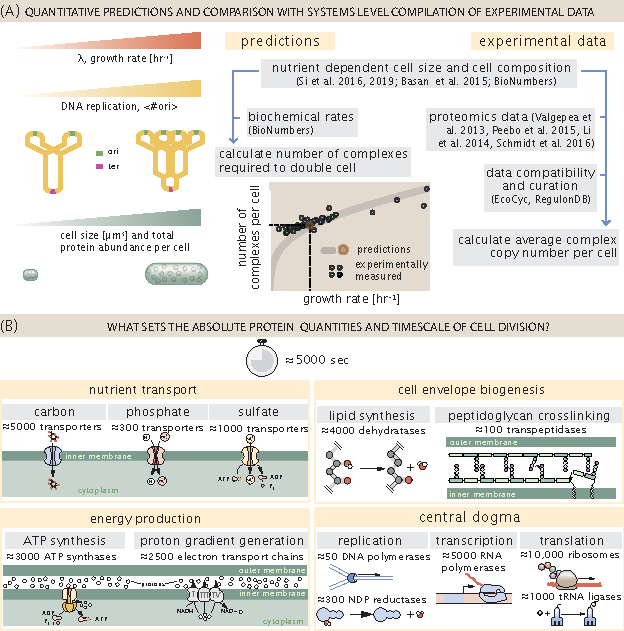
\includegraphics{main_figs/fig1_schematic_categories_grouped.pdf}
    \caption{\textbf{Transport and synthesis processes necessary for cell division.}
            We consider an array of processes necessary for a cell to double its
            molecular components, broadly grouped into four classes. These
            categories are (A) nutrient transport across the cell membrane, (B) cell envelope
            biogenesis, (C) energy production (namely, ATP synthesis), and (D) processes associated with the central dogma.
            Numbers shown are the approximate number of complexes of each type
            observed at a growth rate of 0.5 hr$^{-1}$, or a cell doubling time
            of $\approx$ 5000 s.}
    \label{fig:categories}
    }
\end{figure}

% \section{Nutrient Transport}
In order to build new cellular mass, the molecular and elemental building
blocks must be scavenged from the environment in different forms. Carbon, for
example, is acquired via the transport of carbohydrates and sugar alcohols
with some carbon sources receiving preferential treatment in their
consumption \citep{monod1947}. Phosphorus, sulfur, and nitrogen, on the other
hand, are harvested primarily in the forms of inorganic salts, namely
phosphate, sulfate, and ammonia \citep{jun2018, assentoft2016, stasi2019,
antonenko1997, rosenberg1977, willsky1973}. All of these compounds have
different permeabilities across the cell membrane and most require some
energetic investment either via ATP hydrolysis or through the proton
electrochemical gradient to bring the material across the hydrophobic cell
membrane. Given the diversity of biological transport mechanisms and the vast
number of inputs needed to build a cell, we begin by considering transport of
elemental requirements as a possible rate-limiting step of bacterial cell
division.


The elemental composition of \textit{E. coli} has received much quantitative
attention over the past half century \citep{neidhardt1991, taymaz-nikerel2010,
heldal1985, bauer1976}, providing us a starting point for estimating the
copy numbers of various transporters. While there is some variability in the
exact elemental percentages (with different uncertainties), we can estimate that the
dry mass of a typical \textit{E. coli} cell is $\approx$ 45\% carbon (BNID:
100649, \cite{milo2010}), $\approx$ 15\% nitrogen (BNID: 106666,
\cite{milo2010}), $\approx$ 3\% phosphorus (BNID: 100653, \cite{milo2010}), and
1\% sulfur (BNID: 100655, \cite{milo2010}). In the coming paragraphs, we will examine how many transporters and/or channels
must be present to maintain these elemental compositions with a moderate
doubling time of 6000 s.

\subsection{Carbon Transport}
We begin with the most abundant element by mass, carbon. Using $\approx$ 0.3
pg as the typical \textit{E. coli} dry mass (BNID: 103904, \cite{milo2010}),
we estimate that $\approx 10^{10}$ carbon atoms must be brought into the cell
in order to double all of the carbon-containing molecules (\FIG{carbon_tport}(A,
top))). Typical laboratory
growth conditions, such as those explored in the aforementioned proteomic data
sets, provide carbon as single class of sugar such as glucose, galactose, or
xylose to name a few. \textit{E. coli} has evolved myriad mechanisms by which these sugars can
be transported across the cell membrane. One such mechanism of transport is via
the PTS system which is a highly modular system capable of transporting a diverse
range of sugars \citep{escalante2012}. The glucose-specific
component of this system transports $\approx$ 200 glucose
molecules per second per channel (BNID: 114686, \cite{milo2010}). Making the
assumption that this is a typical sugar transport rate, coupled with the
need to transport 10$^{10}$ carbon atoms, we arrive at the conclusion that on the
order of 1000 transporters must be expressed in order to bring in enough carbon
atoms to divide in 6000 s, diagrammed in the top panel of \FIG{carbon_tport}(A). This estimate, along with the observed average number
of carbohydrate transporters present in the proteomic data sets
\citep{schmidt2016, peebo2015,valgepea2013,li2014}, is shown in
\FIG{carbon_tport}(A). While we estimate 1000 transporters are needed, the
data reveals that at a division time of $\approx 6000$ s there is nearly a
ten-fold excess of transporters. Furthermore, the data illustrates that the
average number of carbohydrate transporters present is largely-growth rate
independent.

\begin{figure}
    \begin{fullwidth}
    \centering{
    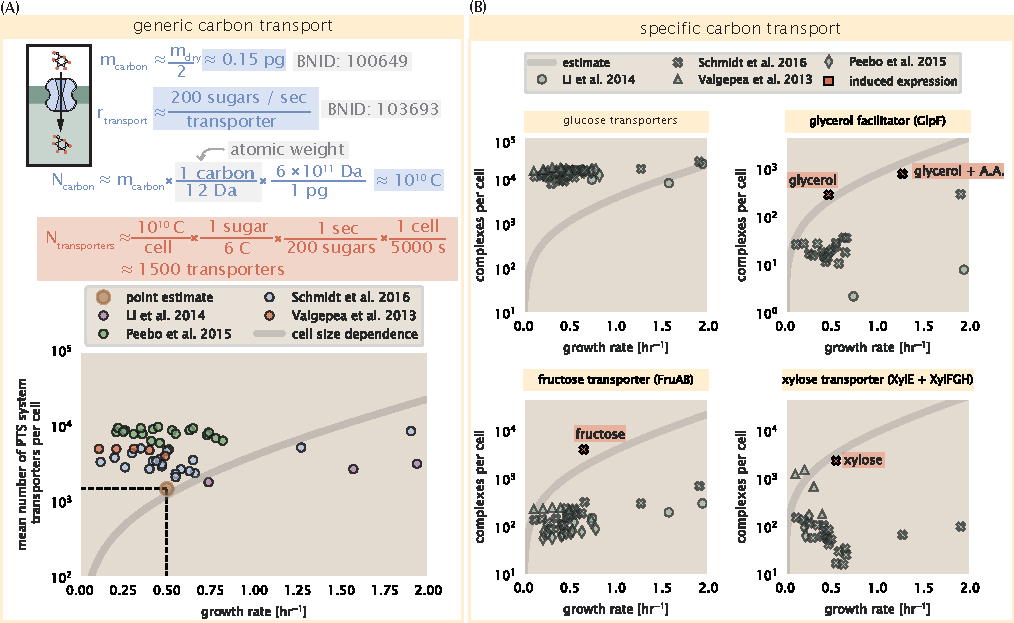
\includegraphics{main_figs/fig2_carbon_transport.pdf}
    \caption{\textbf{The abundance of carbon transport systems across growth
    rates.} (A) A simple estimate for the minimum number of generic carbohydrate
    transport systems (top) assumes $\approx 10^{10}$ C are needed to complete
    division, each transported sugar contains $\approx 6$ C, and each
    transporter conducts sugar molecules at a rate of $\approx 200$ per second.
    Bottom plot shows the estimated number of transporters needed at a growth
    rate of $\approx 0.5 $ per hr (light-brown point and dashed lines). Colored
    points correspond to the mean number of carbohydrate transporters for
    different growth conditions across different published datasets. (B) The
    abundance of various specific carbon transport systems plotted as a function
    of the population growth rate. Red points and red-highlighted text indicate conditions in which the
    only source of carbon in the growth medium induces expression of the
    transport system.}
    \label{fig:carbon_tport}
    }
    \end{fullwidth}
\end{figure}

The estimate presented in \FIG{carbon_tport}(A) neglects any specifics of the
regulation of carbon transport system and presents a data-averaged view of how
many carbohydrate transporters are present on average. Using the diverse array
of growth conditions explored in the proteomic data sets, we can explore how
individual carbon transport systems depend on the population growth rate. In
\FIG{carbon_tport}(B), we show the total number of carbohydrate transporters
specific to different carbon sources. A striking observation, shown in the
top-left plot of \FIG{carbon_tport}(B), is the constancy in the expression of the
glucose-specific transport systems (the PtsG enzyme of the PTS system and the
glucose-transporting ManXYZ complex). Additionally, we note that the total number
of glucose-specific transporters is tightly distributed $\approx 10^4$ per cell,
an order of magnitude beyond the estimate shown in \FIG{carbon_tport}(A). This
illustrates that \textit{E. coli} maintains a substantial number of complexes
present for transporting glucose which is known to be the preferential carbon
source \citep{monod1947, liu2005a, aidelberg2014}.

It is now understood that a large number of metabolic operons are regulated
with dual-input logic gates that are only expressed when glucose
concentrations are low (mediated by cyclic-AMP receptor protein CRP) and the
concentration of other carbon sources are elevated \citep{gama-castro2016, zhang2014a}. A
famed example of such dual-input regulatory logic is in the regulation of the
\textit{lac} operon which is only natively activated in the absence of glucose and the
presence of allolactose, an intermediate in lactose metabolism \citep{jacob1961}, though
we now know of many other such examples \citep{ireland2020, gama-castro2016,
belliveau2018}. This illustrates that once glucose is depleted from the
environment, cells have a means to dramatically increase the abundance of the
specific transporter needed to digest the next sugar that is present. Several
examples of induced expression of a specific carbon-source transporters are
shown in \FIG{carbon_tport}(B). Points colored in red (labeled by red
text-boxes) correspond to growth conditions in which the specific carbon source
(glycerol, xylose, or fructose) is present. These plots show that, in the
absence of the particular carbon source, expression of the transporters is
maintained on the order of $\sim 10^2$ per cell. However, when induced, the
transporters become highly-expressed and are present on the order of $\sim
10^4$ per cell, which exceeds the generic estimate given in
\FIG{carbon_tport}(A). Together, this generic estimation and the specific
examples of induced expression suggest that transport of carbon across the cell
membrane, while critical for growth, is not the rate-limiting step of cell division.

\subsection{Phosphorus and Sulfur Transport}
We now turn our attention towards other essential elements, namely phosphorus and
sulfur. Phosphorus is critical to the cellular energy economy in the form of
high-energy phosphodiester bonds making up DNA, RNA, and the XTP energy pool as
well as playing a critical role in the post-translational modification of
proteins and defining the polar-heads of lipids. In total, phosphorus
makes up $\approx$3\% of the cellular dry mass which in typical experimental conditions is in the form of inorganic phosphate. The cell membrane
has remarkably low permeability to this highly-charged and critical molecule,
therefore requiring the expression of active transport systems. In \textit{E. coli}, the proton
electrochemical gradient across the inner membrane is leveraged to transport
inorganic phosphate into the cell \cite{rosenberg1977}.
Proton-solute symporters are widespread in \textit{E. coli} \cite{ramos1977,
booth1979} and can have rapid transport rates of 50 molecules per second for
sugars and other solutes (BNID: 103159; 111777, \cite{milo2010}). In \textit{E.
coli} the PitA phosphate transport system has been shown to very tightly coupled
with the proton electrochemical gradient with a 1:1 proton:phosphate
stoichiometric ratio \citep{harris2001, feist2007}. Illustrated in
\FIG{phospho_sulfo_tport}(A), we can estimate that $\approx$ 300
phosphate transporters are necessary to maintain an $\approx$ 3\% dry mass with
a 6000 s division time. This estimate is again satisfied when we examine the
observed copy numbers of PitA in proteomic data sets (plot in
\FIG{phospho_sulfo_tport}(A)). While our estimate is very much in line with the
observed numbers, we emphasize that this is likely a slight over estimate of the
number of transporters needed as there are other phosphorous scavenging systems,
such as the ATP-dependent phosphate transporter Pst system which we have neglected.

Satisfied that there are a sufficient number of phosphate transporters
present in the cell, we now turn sulfur transport as another potentially rate
limiting process. Similar to phosphate, sulfate is highly-charged
not particularly membrane permeable, requiring active
transport. While there exists a H+/sulfate symporter in \textit{E.
coli}, it is in relatively low abundance and is not well characterized
\citep{zhang2014}. Sulfate is predominantly acquired via the ATP-dependent ABC
transporter CysUWA system which also plays an important role in selenium
transport \citep{sekowska2000, sirko1995}. While specific kinetic details of
this transport system are not readily available, generic ATP transport
systems in prokaryotes are on the order of 1 to 10 molecules per second
(BNID: 109035, \cite{milo2010}). Combining this generic
transport rate, measurement of sulfur comprising 1\% of dry mass, and a 6000
second division time yields an estimate of $\approx$ 1000 CysUWA
complexes per cell (\FIG{phospho_sulfo_tport}(B)). Once again, this estimate
is in notable agreement with proteomic data sets, suggesting that there are
sufficient transporters present to acquire the necessary sulfur. In a similar
spirit of our estimate of phosphorus transport, we emphasize that this is
likely an overestimate of the number of necessary transporters as we have
neglected other sulfur scavenging systems that are in lower
abundance.


\begin{figure*}
    \begin{fullwidth}
    \centering{
        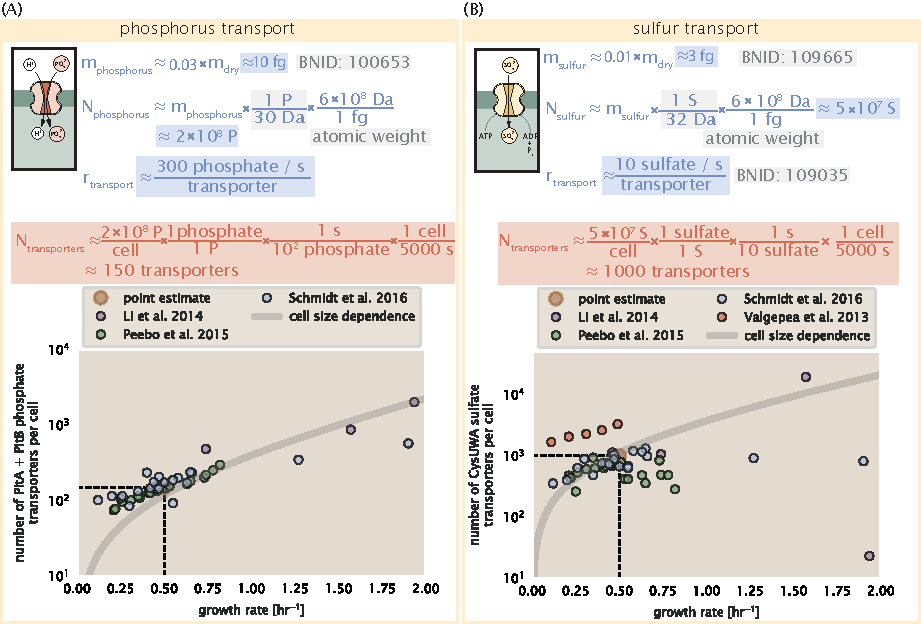
\includegraphics{main_figs/fig3_phospho_sulfo_transport.pdf}
        \caption{\textbf{Estimates and measurements of phosphate and sulfate
        transport systems as a function of growth rate.} (A) Estimate for the
        number of PitA phosphate transport systems needed to maintain a 3\%
        phosphorus \textit{E. coli} dry mass. Points in plot correspond to the
        the total number of PitA transporters per cell. (B) Estimate of the
        number of CysUWA complexes necessary to maintain a 1\% sulfur \textit{E.
        coli} dry mass. Points in plot correspond to average number of CysUWA
        transporter complexes that can be formed given the transporter
        stoichiometry [CysA]$_2$[CysU][CysW][Sbp/CysP].}
        \label{fig:phospho_sulfo_tport}
    }
    \end{fullwidth}
\end{figure*}

\subsection{Nitrogen Transport}
Finally, we turn to nitrogen transport as the last remaining transport system
highlighted in \FIG{categories}. Unlike phosphate, sulfate, and various sugar
molecules, nitrogen in the form of ammonia can readily diffuse across the
cell membrane and has a permeability on par with water ($\approx 10^5$ nm/s,
BNID:110824 \cite{milo2010}). In particularly nitrogen-poor
conditions, \textit{E. coli} expresses a transporter (AmtB) which appears to aid in
nitrogen assimilation, though the mechanism and kinetic details of transport
is still a matter of debate \citep{heeswijk2013a, khademi2004}. Beyond ammonia,
another plentiful source of nitrogen come in the form of glutamate, which has it's
own complex metabolism and scavenging pathways. However, nitrogen is plentiful
in the growth conditions examined in this work, permitting us to neglect
nitrogen transport as a potential rate limiting process in cell division.

\section{Energy Production}
Cells consume and generate energy predominantly in the form of nucleoside
triphosphates (NTPs) in order to grow. The high-energy phosophodiester bonds of
(primarily) ATP power a variety of cellular processes that drive biological
systems away from thermodynamic equilibrium. We now turn to the synthesis of ATP
as a potential process that may limit growth, which also requires us to consider
the maintenance of the electrochemical proton gradient which powers it.

\subsection{ATP Synthesis}
Hydrolysis of the terminal phosphodiester bond of ATP into ADP (or
alternatively GTP and GDP) and an inorganic phosphate provides the
thermodynamic driving force in a wide array of biochemical reactions. One
such reaction is the formation of peptide bonds during translation, which
requires $\approx$ 2 ATPs for the charging of an amino acid to the tRNA and
$\approx$ 2 GTPs for the formation of each peptide bond. Assuming the ATP
costs associated with error correction and post-translational modifications
of proteins are negligible, we can make the approximation that each peptide
bond has a net cost of $\approx$ 4 ATP (BNID: 101442).
Formation of GTP from ATP is achieved via the action of nucleoside
diphosphate kinase, which catalyzes this reaction without an energy
investment \citep{lascu2000} and therefore consider all NTP requirements of
the cell to be functionally equivalent to being exclusively ATP. In total,
the energetic costs of peptide bond formation consume $\approx$ 80\% of the
cells ATP budget [BNID: 107782; 106158; 101637; 111918,
\cite{lynch2015,stouthamer1973}]. The pool of ATP is produced by the
F$_1$-F$_0$ ATP synthase -- a membrane-bound rotary motor which under ideal
conditions can yield $\approx$ 300 ATP per second [BNID: 114701;
\cite{weber2003}].

To estimate the total number of ATP equivalents consumed during a cell cycle, we
will make the approximation that there are $\approx 3\times10^6$ proteins per
cell with an average protein length of $\approx$ 300 peptide bonds (BNID:
115702; 108986; 104877). Taking these values together, coupled with an estimate
of $\approx$ 4 ATP equivalents per peptide bond, we find that the typical
\textit{E. coli} cell consumes $\sim 5 \times 10^9$ ATP per cell cycle on
protein synthesis alone. Assuming that each ATP synthases operates at its
maximal speed (300 ATP per second per synthase), $\approx$ 3000 ATP synthases
are needed to keep up with the energy demands of the cell. This estimate
is comparable with the experimental observations,  shown in
\FIG{energy_production} (A). We note that this estimate assumes all ATP is
synthesized via ATP synthase and neglects synthesis via fermentative metabolism.
This simplification may explain why at the fastest growth rates ($\approx$ 2
hr$^{-1}$), our continuum estimate predicts more synthase than is experimentally
observed (gray line in \FIG{energy_production}). At rapid growth rates,
\textit{E. coli} enters a type of overflow metabolism where fermentative
metabolism becomes pronounced \citep{szenk2017}.

\subsection{Generating the Proton Electrochemical Gradient}
In order to produce ATP, the F$_1$-F$_0$ ATP synthase itself must consume
energy. Rather than burning through its own product (and violating
thermodynamics), this intricate macromolecular machine has evolved to exploit
the electrochemical potential established across the inner membrane through
cellular respiration. This electrochemical gradient is manifest by the pumping
of protons into the intermembrane space via the electron transport chains as
they reduce NADH. In \textit{E. coli}, this potential difference is $\approx
-$200 mV (BNID: 102120). A simple estimate of the inner membrane as a capacitor
with a working voltage of -200 mV reveals that $\approx 2\times 10^4$ protons
must be present in the intermembrane space. However, each rotation of an ATP
synthase shuttles $\approx$ 4 protons into the cytosol (BNID: 103390). With a few thousand ATP
synthases producing ATP at their maximal rate, the potential difference would be
rapidly abolished in a few milliseconds if it were not being actively
maintained.

The electrochemistry of the electron transport complexes of \textit{E. coli}
have been the subject of intense biochemical and biophysical study
\citep{ingledew1984, khademian2017,cox1970,henkel2014}. A recent work
\citep{szenk2017} examined the respiratory capacity of the \textit{E. coli}
electron transport complexes using structural and biochemical data, revealing
that each electron transport chain rapidly pumps protons into the
intermembrane space at a rate of $\approx$ 1500 protons per second (BIND:
114704; 114687). Using our estimate of the number of ATP synthases required
per cell [\FIG{energy_production}(A)], coupled with these recent
measurements, we estimate that $\approx 3000$ electron transport complexes
would be necessary to facilitate the $\sim 5 \times 10^6$ protons per second
diet of the cellular ATP synthases. This estimate is in agreement with the
number of complexes identified in the proteomic datasets [plot in
\FIG{energy_production}(B)]. This suggests that every ATP synthase must be
accompanied by $\approx$ 1 functional electron transport chain.

\begin{figure}
    \begin{fullwidth}
        \centering{
            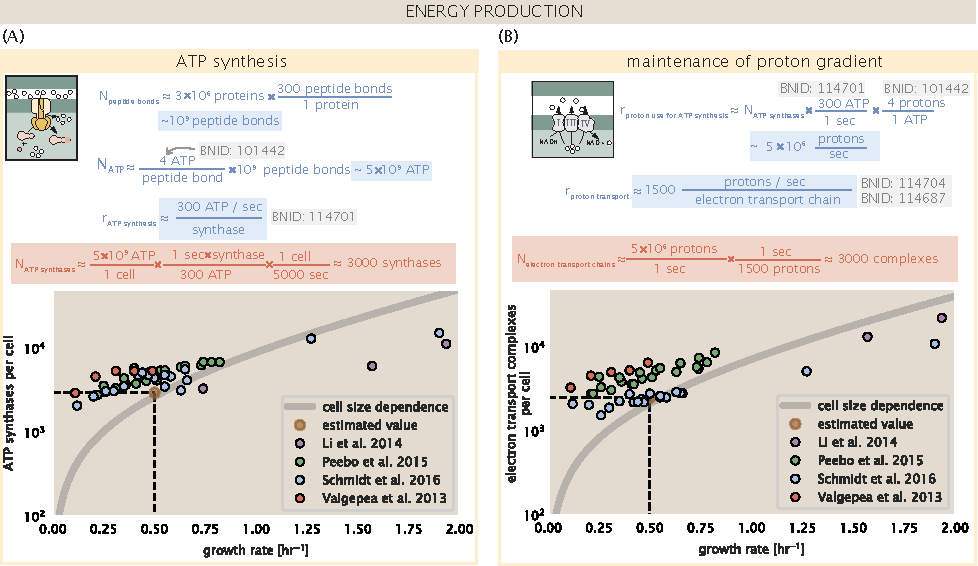
\includegraphics{main_figs/fig4_energy_production.pdf}
            \caption{\textbf{The abundance of F$_1$-F$_0$ ATP synthases and
            electron transport chain complexes as a function of growth
            rate.} (A) Estimate of the number of F$_1$-F$_0$ ATP synthase
            complexes needed to accommodate peptide bond formation and other NTP
            dependent processes. Points in plot correspond to the
            mean number of complete F$_1$-F$_0$ ATP synthase complexes that
            can be formed given proteomic measurements and the subunit
            stoichiometry
            [AtpE]$_{10}$[AtpF]$_2$[AtpB][AtpC][AtpH][AtpA]$_{3}$[AtpG][AtpD]$_3$.
            (B) Estimate of the number of electron transport chain complexes
            needed to maintain a membrane potential of $-$200 mV given
            estimate of number of F$_1$-F$_0$ ATP synthases from (A). Points
            in plot correspond to the average number of complexes identified
            as being involved in aerobic respiration by the Gene Ontology
            identifier GO:0019646 that could be formed given proteomic
            observations. These complexes include cytochromes \textit{bd1}
            ([CydA][CydB][CydX][CydH]), \textit{bdII} ([AppC][AppB]),
            \textit{bo$_3$},([CyoD][CyoA][CyoB][CyoC]) and NADH:quinone
            oxioreducase I
            ([NuoA][NuoH][NuoJ][NuoK][NuoL][NuoM][NuoN][NuoB][NuoC][NuoE][NuoF][NuoG][NuoI])
            and II ([Ndh]). Grey lines in both (A) and (B) correspond to the
            estimate procedure described, but applied to a continuum of growth
            rates. We direct the reader to the Supporting Information for a more
            thorough description of this approach.}
        \label{fig:energy_production}
        }
    \end{fullwidth}
\end{figure}


\subsubsection{Limits on Biosynthesis in a Crowded Membrane}
Our estimates thus far have focused on biochemistry at the periphery of the cell.
Since surface area and volume do not scale identically as cell size changes,  in
order to better understand the physical constraints on transport and  energy
production it is necessary to consider the consequence of a changing S/V
ratio, which will decrease at faster growth rates. Here we use our analysis of
ATP production  to consider this constraint.

In our estimate of ATP production above we found that a cell demands about $5
\times 10^9$ ATP per cell cycle or $10^6$ ATP/s. With a cell volume of roughly 1
fL (BNID: 100004), this corresponds to about $2 \times 10^{10}$ ATP per fL of cell volume, in
line with previous estimates \citep{stouthamer1977, szenk2017}. In
\FIG{energy_scaling} (A) we plot this ATP demand as a function of the S/V ratio
in green, where we have considered a range of cell shapes from spherical to
rod-shaped with an aspect ratio (length/width) equal to 4. In order to consider
the maximum ATP that could be produced, we consider the amount of ATP that can
be generated by a membrane filled with ATP synthase and electron transport
complexes and a maximal production rate of about 3 ATP / (nm$^2 \cdot$s)
\citep{szenk2017}. This is shown in blue in \FIG{energy_scaling}(A), which shows
that at least for the growth rates observed (right column in plot), the energy
demand is roughly an order of magnitude less. Interestingly, \cite{szenk2017}
found that ATP production by respiration is less efficient than by
fermentation on a per membrane area basis, due to the additional proteins of the
electron transport chain. This suggests that, even under anaerobic growth, cells
will have sufficient membrane space for ATP production.

The analysis highlights that there will indeed be a maximum attainable cell size
due to a diminishing capacity to provide resources as the cell increases in
size. The maximum energy production in \FIG{energy_scaling}(A), however, does
represent a somewhat unachievable limit since the inner membrane must also
include other proteins such as those we've considered for nutrient transport and cell
wall biogenesis. To better understand the overall proteomic makeup of the inner
membrane, we therefore used Gene Ontology (GO) annotations \citep{ashburner2000,
thegeneOntologyconsortium2018} to identify all proteins embedded or peripheral
to the inner membrane (GO term: 0005886). Those associated but not
membrane-bound include proteins like MreB and FtsZ and must nonetheless be
considered as a vital component occupying space on the membrane. In
\FIG{energy_scaling}(B), we find that the total protein mass per \textmu m$^2$
is nearly constant across growth rates. Interestingly, when we consider the
distribution of proteins grouped by their Clusters of Orthologous Groups (COG)
\citep{tatusov2000}, the relative abundance for those in metabolism (including
ATP synthesis via respiration) is also relatively constant across growth rates,
suggesting that no one process (energy production, nutrient uptake, etc.) is
particularly dominating even at fast growth rates [\FIG{energy_scaling}(C)].

\begin{figure}
    \begin{fullwidth}
        \centering{
            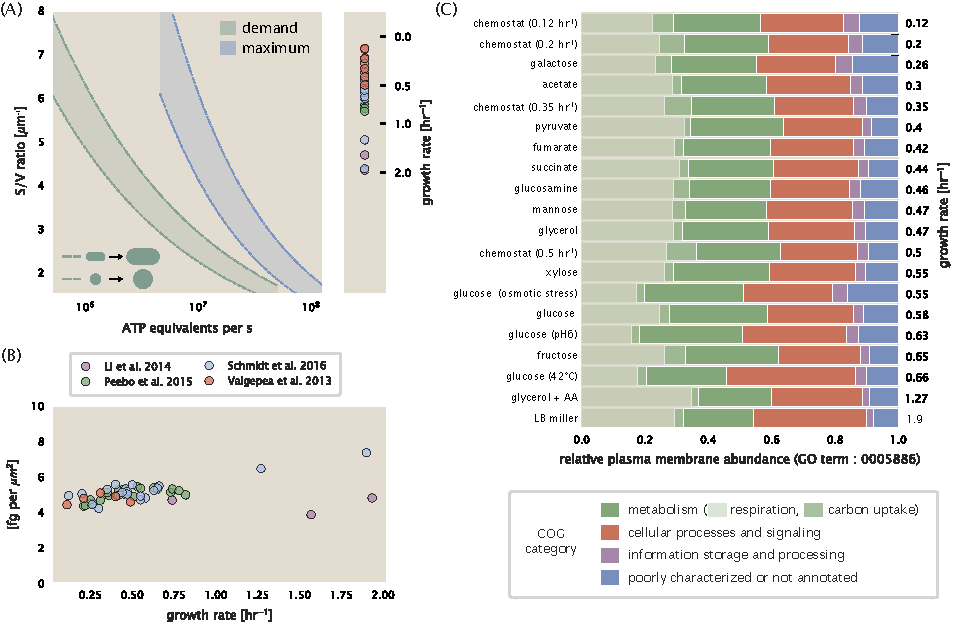
\includegraphics{main_figs/fig5_energy_SV_scaling.pdf}
            \caption{\textbf{Influence of cell size and surface area to volume
            (S/V) ratio on ATP production and inner membrane composition.} (A) Scaling
            of ATP demand and maximum ATP production through respiration as a
            function of S/V ratio. Cell volumes of 0.5 fL to 50 fL were
            considered, with the dashed (\texttt{- -}) line corresponding to a
            sphere and the dash-dot line (\texttt{-.}) reflecting a rod-shaped
            bacterium like \textit{E. coli} with a typical aspect ratio (length
            / width) of 4 \citep{shi2018}. The ATP demand is calculated as
            $10^6$ ATP/(\textmu m$^3$ s), while the maximum ATP production rate
            is taken to be 3 ATP / (nm$^2 \cdot$s)
            \citep{szenk2017}, with calculations of \textit{E. coli} volume and
            surface area detailed in Appendix \nameref{sec:protein_size_SV}. In
            this calculation, 50\% of the bacterial inner membrane is assumed to
            be protein, with the remainder lipid. (B) Total protein mass per
            \textmu m$^2$ calculated for proteins with inner membrane annotation
            (GO term: 0005886). (C) Relative protein abundances by mass based on
            COG annotation. Metabolic proteins are further separated into
            respiration (F$_1$-F$_0$ ATP synthase, NADH dehydrogenase I,
            succinate:quinone oxidoreductase, cytochrome bo$_3$ ubiquinol
            oxidase, cytochrome bd-I ubiquinol oxidase) and carbohydrate
            transport (GO term: GO:0008643). Note that the elongation factor
            EF-Tu can also associate with the inner membrane, but was excluded
            in this analysis due to its high relative abundance (roughly
            identical to the summed protein shown in part
            (B)).}\label{fig:energy_scaling}
            }
                \end{fullwidth}
\end{figure}

% \section{Synthesis of the Cell Envelope}
The subjects of our estimates thus far have been localized to the periphery of
the cell, embedded within the hydrophobic lipid bilayer of the inner membrane.
As outlined in \FIG{energy_scaling}, cells could in principle increase the
expression of the membrane-bound ATP synthases and electron transport chains to
support a larger energy budget across a wide range of cell volumes and membrane
surface areas. This ability, however, is contingent on the ability for the cell
to expand the surface area of the cell by synthesizing new lipids as well as
expanding the peptidoglycan cell wall. In this next class of estimates, we will
turn our focus to these process and consider the copy numbers of the relevant
proteinaceous components needed to synthesize lipids and form new cell wall
material. 

\subsection{Lipid Synthesis}
The cell envelopes of gram negative bacteria (such as \textit{E. coli}) are
composed of an inner and outer phospholipid bilayer membrane separated by a
$\approx 10$ nm periplasmic space. As mentioned in our discussion of the
surface area to volume constraints on energy production, \textit{E. coli} is
a rod-shaped bacterium with a 4:1 length-to-width aspect ratio. At modest
growth rates, such as our stopwatch of 5000 s, the total cell surface area is
$\approx$ 5 \textmu m$^2$ (BNID: 101792, \cite{milo2010}). As there are two
membranes, each of which composed of two lipid leaflets, the total membrane
area is $\approx 20$\textmu m$^2$, a remarkable value compared to the
$\approx$ 2\textmu m length of the cell.

While this represents the total area of the membrane, this does not mean that it
is composed entirely of lipid molecules. Rather the dense packing of the
membrane with proteins means that only $\approx$ 40 \% of the membrane area is
occupied by lipids (BNID: 100078, \cite{milo2010}). Using a rule-of-thumb of 0.5
nm$^2$ as the surface area of the typical lipid (BNID: 106993, \cite{milo2010}),
we arrive at an estimate of $\approx$ 2 $\times$ 10$^7$ lipids per cell, an
estimate in close agreement with experimental measurements (BNID: 100071,
102996; \cite{milo2010}).

The membranes of \textit{E. coli} are composed of a variety of different
lipids, each of which unique in their structures and biosynthetic pathways
\citep{sohlenkamp2016}. With such diversity in biosynthesis, it becomes
difficult to identify which step(s) may be the rate-limiting reactions. This
objective is further complicated by sparsity of \textit{in vivo} kinetic
data. Recently, a combination of stochastic kinetic modeling
\citep{ruppe2018} and \textit{in vitro} kinetic measurements
\citep{ranganathan2012, yu2011} have revealed remarkably slow steps in the
fatty acid synthesis pathways which may serve as the rate limiting reactions.
One such step is the removal of hydroxyl groups from the fatty-acid chain by
ACP dehydratase, leading to the formation of carbon-carbon double bonds. This
reaction, catalyzed both by proteins FabZ and FabA in \textit{E. coli}
\citep{yu2011}, have been estimated to have kinetic turnover rates of
$\approx$ 1 dehydration per second per enzyme \citep{ruppe2018}. Combining
this rate estimate, our previous estimates for the number of lipids to be
formed, and a 5000 second division yields and estimate that the cell requires
$\approx$ 4000 ACP dehydratases. This estimate is in reasonable agreement with the experimentally observed copy
numbers of FabZ and FabA (\FIG{cell_envelope}(A)). Furthermore, we can extend
this estimate to account for the change in membrane surface area as a function
of the growth rate (grey line in \FIG{cell_envelope}(A)), which captures the
observed growth rate dependent expression of these two enzymes. 

Despite the slow catalytic rate of the FabZ and FabA enzymes, we argue that the
generation of fatty acids is not a bottleneck in cell division and is not the
key process responsible for setting the bacterial growth rate. Experimental
evidence has shown that the rate of fatty-acid synthesis can be drastically
increased \textit{in vitro} by increasing the concentration of FabZ
\cite{yu2011}. Stochastic simulations of the complete fatty acid synthesis
pathway of \textit{E. coli} further supports this experimental observation
\cite{ruppe2018}. Thus, if this step was the determining factor in cell
division, increasing growth rate could be as simple as increasing the number of
ACP dehydratases per cell. With a proteome size of $\approx$ 3$\times$10$^6$
proteins, a drastic increase in expression from 4000 to 40,000 ACP dehydratases
would result in a $\approx$ 1\% increase in the proteome pool. As other proteins
such as ribosomes and tRNA synthetases are in much larger
abundance than 4000 per cell (as we will see in the coming sections), it is
unlikely that expression of ACP dehydratases couldn't be increased to facilitate
faster growth.


\begin{figure}
    \begin{fullwidth}
    \centering{
        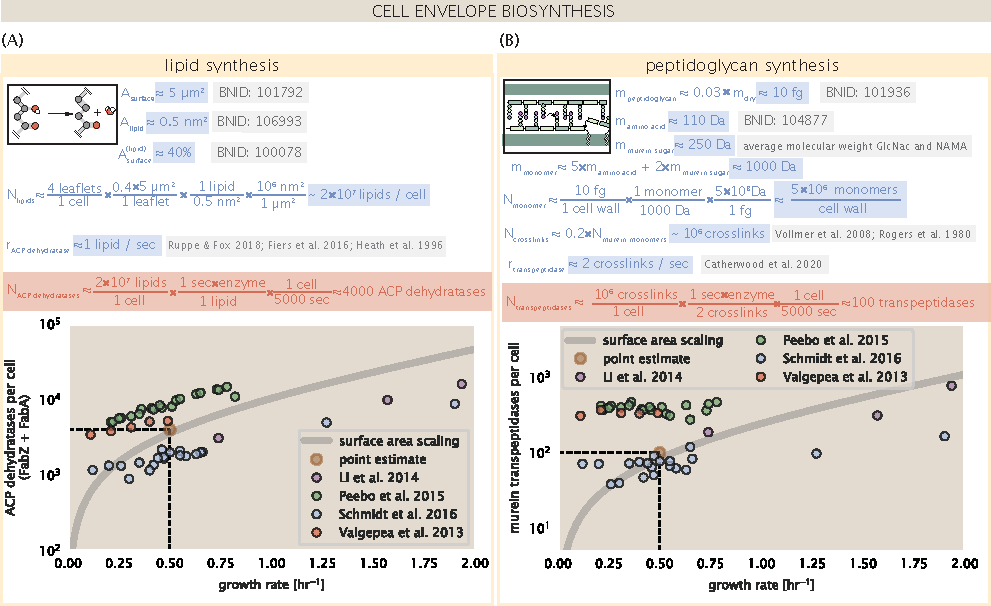
\includegraphics{main_figs/cell_wall_peptidoglycan.pdf}
        \caption{\textbf{Estimation of the key components involved in cell
        envelope biosynthesis.} (A) Top panel shows a schematic estimation for
        the number of ACP dehydratases necessary to form functional
        phospholipids. The rate of ACP dehydratases was inferred from
        experimental measurements via a stochastic kinetic model described in
        \cite{ruppe2018}. Bottom panel shows the experimentally observed complex
        copy numbers using the stoichiometries [FabA]$_2$ and [FabZ]$_2$. (B) An
        estimate for the number of peptidoglycan transpeptidases needed to
        complete maturation of the peptidoglycan. The mass of the murein monomer
        was estimated by approximating each amino acid in the pentapeptide chain
        as having a mass of 110 Da and each sugar in the disaccharide having a
        mass of $\approx$ 250 Da. The \textit{in vivo} rate of transpeptidation
        rein \textit{E. coli} was taken from recent analysis by
        \cite{catherwood2020}. The bottom panel shows experimental measurements
        of the transpeptidase complexes in \textit{E. coli} following the
        stoichiometries [MrcA]$_2$, [MrcB]$_2$, [MrdA]$_1$, and [MrdB]$_1$. Grey
        curves in each plot show the estimated number of complexes needed to
        satisfy the synthesis requirements scaled by the surface area as a
        function of growth rate. We direct the reader to the supplemental
        information for a more detailed discussion of this estimate. 
        }
        \label{fig:cell_envelope}
    }
    \end{fullwidth}

\end{figure}


\subsection{Peptidoglycan Synthesis}
While variation in cell size as a function growth rate can be large,
bacterial cells demonstrate exquisite control over their cell shape. The
maintenance of cell shape is due primarily to the intricate meshwork of the
cell wall, a shell of polymerized discaccharides interspersed with short
peptide crosslinks termed the peptidoglycan. In gram negative bacteria, such as \textit{E. coli}, this
enormous peptidoglycan molecule is a few nanometers thick and resides within the
periplasmic space between the inner and outer membrane. The formation of the
peptidoglycan is an intricate process, involving the bacterial actin homolog
MreB \citep{shi2018} along with a variety of membrane-bound and periplasmic
enzymes \citep{morgenstein2015}. The coordinated action of these components
result in a highly-robust polymerization framework which maintains cell shape
even in the face of large-scale perturbations and can restore rod-shaped
morphology even after digestion of the peptidoglycan \citep{harris2018,shi2018}.

In glucose-supported balanced growth, the peptidoglycan alone comprises
$\approx$ 3\% of the cellular dry mass (BNID: 101936, \cite{milo2010}), making it the most massive molecule in
\textit{E. coli}. The polymerized unit of the peptidoglycan is a
N-acetylglucosamine and N-acetylmuramic acid disaccharide, the former of which
is functionalized with a short pentapeptide. With a mass of $\approx$ 1000 Da,
this unit, which we refer to as a murein monomer, is polymerized to form long
strands in the periplasm which are attached to eachother via the peptide linkers. Using the
aforementioned measurement that $\approx$ 3\% of the dry mass is peptidoglycan,
it can be estimated that the peptidoglycan is composed of $\approx$
6$\times$10$^6$ murein monomers.

In principle, each one of these murein monomers can be crosslinked to another
glycan strand via the pentapeptide. In some species, such as in gram-positive
bacterium \textit{Staphylococcus aureus}, the extent of crosslinking can be
large with $>$ 90\% of pentapeptides forming a connection between glycan
strands. In \textit{E. coli}, however, a much smaller proportion ($\approx$
20\%) of the peptides are crosslinked, resulting in a weaker and more porous
cell wall \cite{vollmer2008a, rogers1980}. The formation of these crosslinks
primarily occur during the polymerization of the murein monomers and is
facilitated by a family of enzymes called transpeptidases. In \textit{E. coli},
there are four primary transpeptidases that are involved in lateral and
longitudinal extension of the peptidoglycan. These transpeptidases have only
recently been quantitatively characterized \textit{in vivo} via liquid
chromatography mass spectrometry \citep{catherwood2020}, which revealed a
kinetic turnover rate of $\approx 1 - 2$ crosslinking reactions formed per
second per enzyme.

Pulling these measurements together permits us to make an estimate that on the
order of $\approx$ 100 transpeptidases are needed for complete maturation of the
peptidoglycan, given a division time of $\approx$ 5000 seconds, a value that is
closely aligned with the experimental observations (\FIG{cell_envelope}(B)). Expanding this
estimate to account for the changing volume of the peptidoglycan as a function
of growth rates (grey line in \FIG{cell_envelope}(B)) also qualitatively captures the observed
dependence in the data, though systematic disagreements between the different
data sets makes the comparison more difficult. 

Much as in the case of fatty acid synthesis, we find it unlikely that the
formation of peptidoglycan is a rate limiting step in bacterial cell division.
The estimate we have presented considers only the transpeptidase enzymes that
are involved lateral and longitudinal elongation of the peptidoglycan (proteins
MrdA, MrdB, MrcA, and MrcB). This neglects the presence of other transpeptidases
that are present in the periplasm that are involved in remodeling and maturation
of the peptidoglycan. It is therefore possible that if this was setting the
speed limit for cell division, the simple expression of more maturation
transpeptidases may be sufficient to maintain the structural integrity of the
cell wall. 

Furthermore, it has been shown experimentally that, while critical for cell
wall formation, there are components needed beyond  the transpeptidases to
maintain cell shape and permit cell division. For example, the bacterial actin
homolog MreB polymerizes laterally along the inner membrane and facilitates the
longitudinal expansion of the peptidoglycan. Inhibition of MreB through the
addition of small molecules results in loss of the cell shape, though formation
of the peptidoglycan is not significantly hindered \cite{shi2018}. This suggests
that in considering the development of the cell envelope, proper assembly may
be a more important property to consider beyond synthesis of the appropriate
number of glycan polymers. 
\section{Processes of the Central Dogma}
Up to this point, we have considered a variety of transport and biosynthetic
processes that are critical to acquiring and generating new cell mass. While
there are of course many other metabolic processes we could consider, we now
turn our focus to some of the most important processes which \textit{must} be
undertaken irrespective of the growth conditions -- those of the central
dogma.

\subsection{DNA Replication}
Most bacteria (including \textit{E. coli}) harbor a single, circular chromosome
and can have extra-chromosomal plasmids up to $\sim$ 100 kbp in length. While
we consider the starting material dNTPs in \FIGSUPP[DNA_synthesis]{dntp} and
discussed further in the Appendix Section "\nameref{sec:SI_central_dogma}", here we focus
our quantitative thinking on the chromosome of \textit{E. coli}, which
harbors $\approx$ 5000 genes and $\approx 5\times 10^6$ base pairs.

To successfully divide and produce viable progeny, this chromosome must be
faithfully replicated and segregated into each nascent cell. Replication is
initiated at a single region of the chromosome termed the \textit{oriC} locus
where a pair of replisomes, each consisting of two DNA polymerase III,
begin their high-fidelity replication of the genome in opposite directions
\citep{fijalkowska2012}. \textit{In vitro} measurements have shown that DNA
Polymerase III copies DNA at a rate of $\approx 600$ nucleotides per second
(BNID: 104120). Therefore, to replicate a single chromosome, two replisomes
moving at their maximal rate would copy the entire genome in $\approx$ 4000
s. Thus, with a division time of 5000 seconds, there is sufficient time for a pair
of replisomes complexes to replicate the entire genome.

\begin{figure}
  \centering{
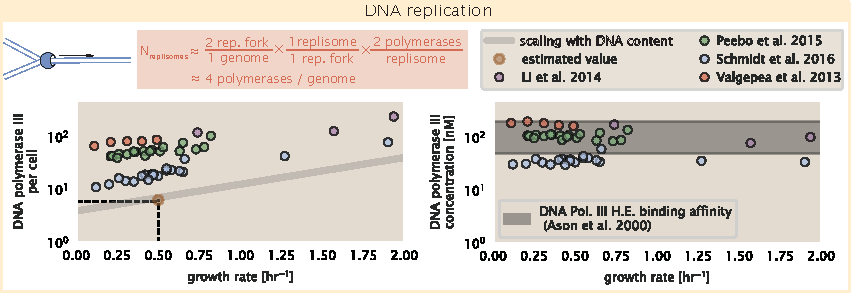
\includegraphics{main_figs/fig6_DNA_replication_main.pdf}
\caption{\textbf{Complex abundance estimates for dNTP synthesis and DNA
replication.} An estimate
for the minimum number of DNA polymerase holoenzyme complexes needed to
facilitate replication of a single genome. Points in the left-hand plot correspond
to the total number of DNA polymerase III holoenzyme complexes
([DnaE]$_3$[DnaQ]$_3$[HolE]$_3$[DnaX]$_5$[HolB][HolA][DnaN]$_4$[HolC]$_4$[HolD]$_4$)
per cell. Right-hand plot shows the effective concentration of DNA polymerase III
holoenzyme (See Appendix \nameref{sec:protein_size_SV} for calculation of cell
size). Grey lines in left-hand panel show the estimated number of
complexes needed as a function of growth, the details of which are described
in the Supplemental Information.} \label{fig:DNA_synthesis}
 }
\figsupp[Estimate and observations of the abundance of ribonucleotide
reductase, a key component in dNTP synthesis.]{Estimate of the number of
ribonucleotide reductase enzymes needed to facilitate the synthesis of
$\approx 10^7$ dNTPs over the course of a 5000 second generation time. Points
in the plot correspond to the total number of ribonucleotide reductase I
([NrdA]$_2$[NrdB]$_2$) and ribonucleotide reductase II ([NrdE]$_2$[NrdF]$_2$)
complexes. Grey lines in top panel show the estimated number of complexes
needed as a function of growth, the details of which are described in the
Appendix.}{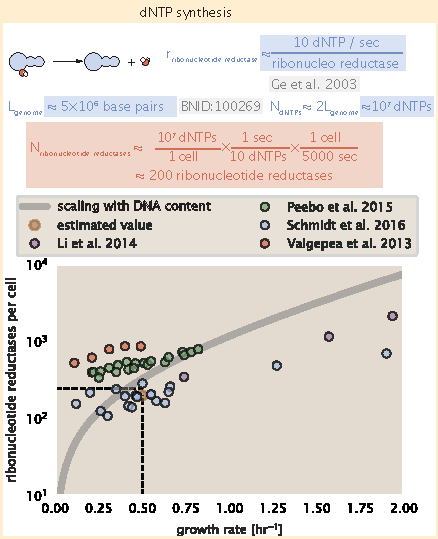
\includegraphics{main_figs/fig6-S1_dNTP_synthesis.pdf}}\label{figsupp:dntp}

\end{figure}

In rapidly growing cultures, bacteria like \textit{E. coli}
can initiate as many as 10 - 12 replication forks at a
given time \citep{bremer2008, si2017},  we expect only a few DNA polymerases
($\approx 10$) are needed. However, as shown in \FIG{DNA_synthesis}, DNA
polymerase III is nearly an order of magnitude more abundant. This discrepancy
can be understood by considering its binding constant to DNA. \textit{In vitro} characterization has quantified the $K_D$ of
DNA polymerase III holoenzyme to single-stranded and double-stranded DNA to be
50 and 200 nM, respectively \citep{ason2000}. The right-hand plot in
\FIG{DNA_synthesis} shows that the concentration of DNA polymerase III
across all data sets is within this range. Thus, its copy number appears to vary such that its
concentration is approximately equal to the dissociation constant to the DNA.
While the processes regulating the initiation of DNA replication are complex and
involve more than just the holoenzyme, these data indicate that the kinetics of
replication rather than the explicit copy number of the DNA polymerase III
holoenzyme is the more relevant feature of DNA replication to consider. In light
of this, the data in \FIG{DNA_synthesis} suggests that for bacteria like
\textit{E. coli}, DNA replication does not represent a rate-limiting step in
cell division. However, it is worth noting that for bacterium like \textit{C.
crescentus} whose chromosomal replication is initiated only once per cell cycle
\citep{jensen2001}, the time to double their chromosome indeed represents an
upper limit to their growth rate.

% \section{Protein synthesis}

Lastly, we turn our attention to the process of translation. So far our
estimates have led to protein copy numbers that are consistent with the
proteomic data, or even in excess of what might be needed for each task under
limiting growth conditions. Even in our example of \textit{E. coli} grown under
different carbohydrate sources (\FIG{carbon_tport}(B)), cells can utilize
alternative carbon sources by inducing the expression of additional membrane
transporters and enzymes. Optimal resource allocation and the role of ribosomal
proteins have been an area of intense quantitative study over the last decade by
Hwa and others \citep{scott2010, hui2015}. From the perspective of limiting
growth, our earlier estimate of rRNA highlighted the necessity for multiple
copies of rRNA genes in order to make enough rRNA, suggesting the possibility
that synthesis of ribosomes might be rate limiting. While the transcriptional
demand for  the ribosomal proteins is substantially lower than rRNA genes, since
many proteins can be translated from relatively fewer mRNA, other ribosomal
proteins like the translation elongation factor EF-Tu also present a substantial
burden. For EF-Tu  in particular, it is the most highly expressed protein in
\textit{E. coli} and  is expressed by multiple genes on the chromosome, tufA and
tufB.

% Experimentally,
% consecutive deletion of rRNA operons showed a significant reduction in growth
% rate in rich media when cells had only 3 or less \citep{levin2017}.

% Separately, it has been found that gross
% overexpression of a protein can dramatically lower growth rate due to the
% altered allocation of resources \citep{basan2015}.

We begin by first estimating the number of tRNA synthetases and ribosomes
required for  a doubling time of 5000 seconds.  \textit{E. coli} has roughly 3 x
10$^6$ proteins per cell, which for an average protein of 300 aa, amounts to the formation
of $\approx$ 10$^9$ peptide bonds. This also corresponds to the
number of amino-acyl tRNA that are used by ribosomes, with the pool of tRNA continuously
recharging new amino acids by tRNA synthetases. At a rate of charging of
about 20 amino-acyl tRNA per second (BNID: 105279, \cite{milo2010}), we find
that cells have more than sufficient tRNA synthetases to meet the demand of
ribosomes during  protein synthesis (\FIG{protein_synthesis}(A)).
If we consider an elongation rate of $\approx$ 15 peptide bonds per second
(BNID: 114271, \cite{milo2010, dai2016}), the formation of $\approx$ 10$^9$
peptide bonds would require 1.5 x 10$^4$ ribosomes at a growth rate of 0.5
hr$^{-1}$. This is indeed consistent with the experimental data shown in
\FIG{protein_synthesis}(B).

[NB: How about moving this estimates paragraph and associated \FIG{protein_synthesis} to SI after all?]

\begin{figure}
    \begin{fullwidth}
    \centering{
        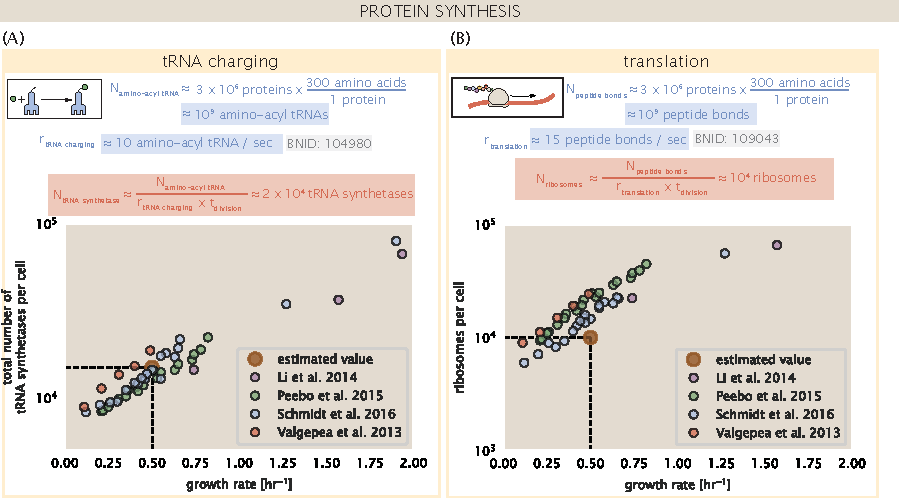
\includegraphics{main_figs/protein_synthesis.pdf}
        \caption{\textbf{Estimation of the required tRNA synthetases and
        ribosomes.} (A) Estimation for the
        number of tRNA synthetases that will supply the required amino acid
        demand. The sum of all tRNA synthetases copy numbers are plotted as a
        function of growth rate ([ArgS], [CysS], [GlnS], [GltX], [IleS], [LeuS],
        [ValS], [AlaS]$_2$, [AsnS]$_2$, [AspS]$_2$, [TyrS]$_2$, [TrpS]$_2$,
        [ThrS]$_2$, [SerS]$_2$, [ProS]$_2$, [PheS]$_2$[PheT]$_2$, [MetG]$_2$,
        [lysS]$_2$, [HisS]$_2$, [GlyS]$_2$[GlyQ]$_2$). (B) Estimation for the
        number of ribosomes required to synthesize all proteins in the cell. The
        average abundance of ribosomes is plotted as a function of growth rate.
        Our estimated values are shown for a growth rate of 0.5 hr$^{-1}$.}
    \label{fig:protein_synthesis}
    }
    \end{fullwidth}
\end{figure}

We can begin to gain some intuition into how translation might limit growth by
noting that the total number of peptide bonds generated as the cell doubles,
$N_{aa}$, which we used in our calculation above, will be given by, $\tau \cdot
r_t \cdot R$. Here, $\tau$ refers to the doubling time of the cell under
steady-state growth, $r_t$ is the maximum translation elongation rate, and $R$
is the average number of ribosomes per cell. With the growth rate related to the
cell doubling time by $\lambda = ln(2)/\tau$, we can write the
translation-limited growth rate as,

\begin{equation}
\lambda_{\textrm{translation-limited}} = \frac{ln(2) \cdot r_t \cdot R}{N_{aa}}.
\end{equation}
Alternatively, since $N_{aa}$ is related to the total protein mass through the
molecular weight of each protein, we can also consider the growth rate in terms
of ribosomal mass fraction. By making the approximation that an average amino
acid has a molecular weight of 110 Da (see \FIG{translation_1}(A)), we can
rewrite the growth rate as,

\begin{equation}
\lambda_{\textrm{translation-limited}} \approx \frac{ln(2) \cdot r_t}{L_R}  \Phi_R,
\label{eq:translation_limit_growth_rate}
\end{equation}
where $L_R$ is the total length in amino acids that make up a ribosome, and
$\Phi_R$ is the ribosomal mass fraction. This is plotted as a function of
ribosomal fraction $\Phi_R$ in \FIG{translation_1}(A), where we take $L_R
\approx $7459 aa, corresponding to the length in amino acids for all ribosomal
subunits of the 50S and 30S complex. This formulation assumes that the cell can
transcribe the required amount of rRNA, which appears reasonable for  \textit{E.
coli} under the  allowing us to consider the inherent limit on growth set by the
ribosome.

The growth rate defined by Equation \ref{eq:translation_limit_growth_rate}
reflects  mass-balance under steady-state growth and has long provided a
rationalization to the apparent linear increase in \textit{E. coli}'s ribosomal
content as a function of growth rate \citep{Goldberger1979, scott2010}. For our
purposes, there are several important consequences of this  trend. Perhaps the
first thing to notice is that there is a maximum growth rate at about $\lambda
\approx 6 hr^{-1}$, or doubling time of about 7 minutes (dashed line). This
growth rate can be viewed as an inherent maximum growth rate due to the need for
the cell to double the cell's entire ribosomal mass. Interestingly, this limit
is independent of the absolute number of ribosomes, but rather is simply given
by time to translate an entire ribosome, $L_R/ r_t$. As shown in
\FIG{translation_1}(B), we can reconcile this with the observation that in order
to double the average number of ribosomes, each ribosome must produce a second
ribosome. This is a process that cannot be parallelized.

For reasonable values of $\Phi_R$, between about 0.1 - 0.3 \citep{scott2010},
the maximum growth rate is in line with experimentally reported growth rates
around 0.5 - 2 $hr^{-1}$. Here we are implicitly assuming that translation
proceeds randomly, without preference between ribosomal or non-ribosomal mRNA,
which appears reasonable. Importantly, in order for a cell to scale this growth
limit set by $\Phi_R$, cells \textit{must} increase their ribosomal abundance.
This can be achieved by either synthesizing more ribosomes or reducing the
fraction of non-ribosomal proteins. Reduction of non-ribosomal proteins is not
straight forward since, as we have found throughout our estimates, doubling a
cell requires a substantial number of other enzymes and transporters. Increasing
the absolute ribosomal abundance is limited by the number of rRNA operons.

\begin{figure}
  \begin{fullwidth}
        \centering{
            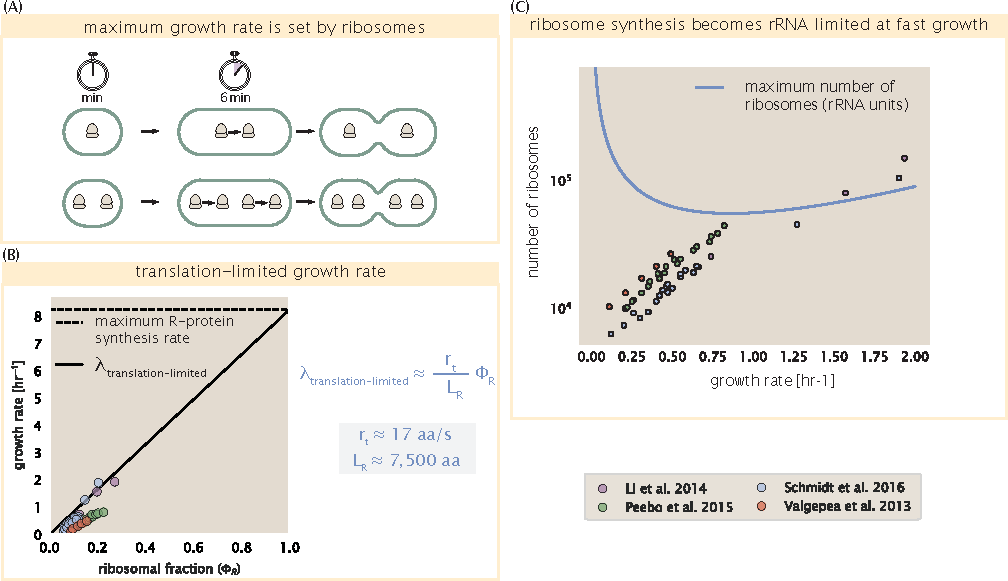
\includegraphics{main_figs/fig7_ribosome_growth_limit_2.pdf}
            \caption{\textbf{Translation-limited growth rate.} (A) Here we
            consider the translation-limited growth as a function of ribosomal
            fraction. By mass balance, the time required to double the entire
            proteome ($N_{aa}$ /$r_t \cdot $) sets the translation-limited
            growth rate, $\lambda_{\textrm{translation-limited}}$. Here $N_{aa}$
            is effectively the number of peptide bonds that must be translated,
            $r_t$ is the translation elongation rate, and $R$ is the number of
            ribosomes. This can also be re-written in terms of the ribosomal
            mass fraction $\Phi_R = m_R$ / $m_{\textrm{protein}}$, where $m_R$
            is the total ribosomal mass and $m_{\textrm{protein}}$ is the mass
            of all proteins in the cell. $L_R$ refers to the summed length of
            the ribosome in amino acids.
            $\lambda_{\textrm{translation-limited}}$ is ploted as a function of
            $\Phi_R$ (solid line). (B) The dashed line in part (A) identifies a
            maximum growth rate that is set by the ribosome. Specifically, this
            growth rate corresponds to the time required to  translation an
            entire ribosome, $L_R/ r_t$ . This is a result that is independent
            of the number of ribosomes in the cell as shown schematically here.
            (C) Schematic showing translation-specific requirements for maintenance
            of steady-state growth. In a nutrient rich environment, amino acid supply $r_{aa}$ is sufficiently in
            excess of demand by ribosomes translating at their maximal rate. In poorer
            nutrient conditions, reduced amino acid supply $r_{aa}$ will decrease
            the rate of elongation. In a regime where $r_{aa}$ is less than $r_t \cdot R$,
            the number of actively translating ribosomes will need to be reduced in order
            to maintain steady-state growth.}
        \label{fig:translation_1}
        }
  \end{fullwidth}
\end{figure}

While it is common for bacteria to decrease their ribosomal abundance in poorer
nutrient conditions \cite{scott2010, liebermeister2014}, this does not decrease
to zero. From the perspective of a bacterium dealing with uncertain nutrient
conditions, there is likely a benefit for the cell to maintain some relative
fraction of ribosomes to support rapid growth as nutrient conditions improve.
However, if we consider a scenario where nutrient conditions become poorer and
poorer, there will be a regime where ribosomes are in excess of the nutrient
supply. If the cell is to maintain steady-state growth, it will need to
attenuate its translational activity since ribosomes would otherwise exhaust
their supply of amino acids and bring cell growth to a halt
(\FIG{translation_1}(C)). In the next section we will consider this more
specifically for \textit{E. coli}, which has been shown to maintain a relatively
high elongation rate even in stationary phase ($\approx$ 8 aa/s, \cite{dai2016})
where cell growth is minimal.

[NB: I'm considering moving this paragraph near the end of the next section].

% In addition,
% given their massive size at about 850 kDa, they may play an as-yet fully
% understood role as a crowding agent in cellular function \cite{delarue2018,
% solerbistue2020}.

\subsection{Multiple replication forks bias ribosome abundance.}

\textit{E. coli} cells grow by an adder mechanism, whereby cells add a constant
volume with each cell division \citep{taheriaraghi2015}. In conjunction with
this, additional rounds of DNA replication are triggered when cells reach a
critical volume per origin of replication (\FIG{translation_ecoli}(A)). This
leads to the classically-described exponential increase in cell size with growth
rate \cite{schaechter1958, si2017, si2019}. In the context of maximizing growth
rate, it is notable that the majority of ribosomal proteins and rRNA operons are
found closer to the DNA origin. Given the need to increase to total gene dosage
of rRNA operons at faster growth rates, and the intimate relationship between ribosomal
content and growth rate we considered above, this raises the possibility that the
observed size scaling and increase in chromosomal content might simply be
a means for the cell to tune biosynthesis according to its
physiological state.

While an increase in transcription has been observed for genes near the origin
in rapidly growing \textit{E. coli}  \citep{scholz2019}, we were unaware of such
characterization at the proteomic level. In order to test whether there is a
relative increase in protein expression for genes closer to the origin, we
calculated a running boxcar average of protein copy number as a function of
each gene's transcriptional start site. While absolute protein copy numbers can vary
substantially across the chromosome, we indeed observe a bias in expression
under fast growth conditions (\FIG{translation_ecoli}(B), showing the result
using a 0.5 kb averaging window). The dramatic change in protein copy number
near the origin mainly reflects the increase in ribosomal protein expression.
This trend is in contrast to slower growth conditions where the average copy
number is more uniform across the length of the chromosome.

\begin{figure*}
    \begin{fullwidth}
    \centering{
        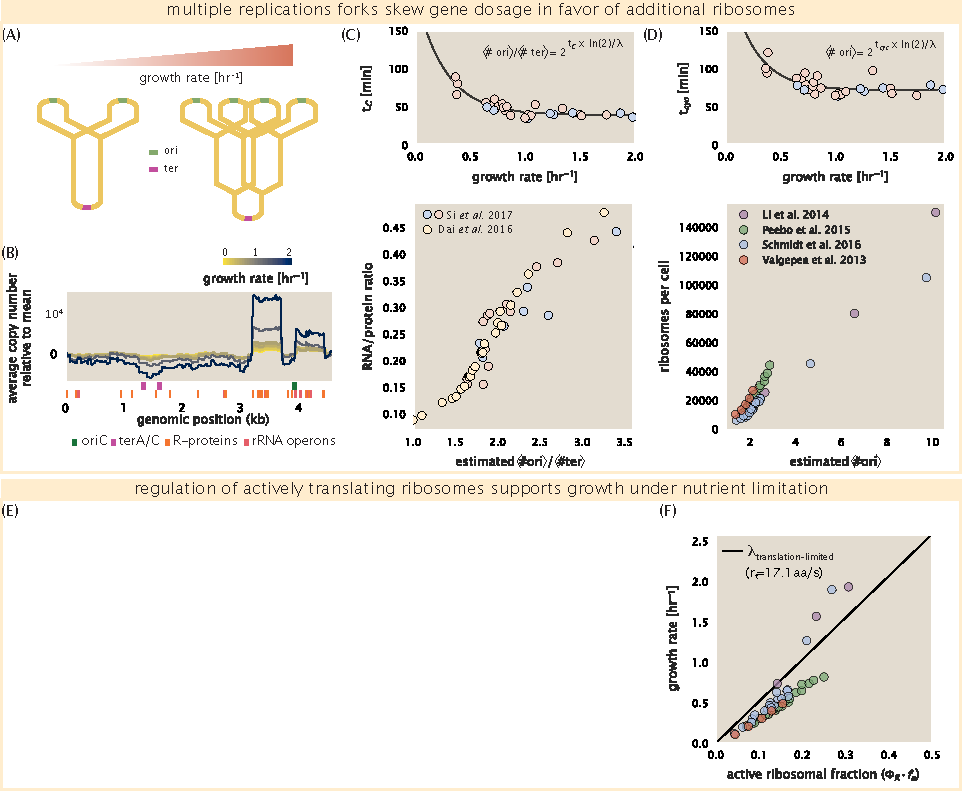
\includegraphics{main_figs/fig8_ribosome_growth_limit_ecoli_temp.pdf}
        \caption{\textbf{Multiple replication forks skew gene dosage and
        ribosomal content.} (A) Schematic shows the expected
        increase in replication forks (or number of ori regions) as \textit{E. coli} cells
        grow faster. (B) A running boxcar average of protein copy number is calculated for
        each each growth condition considered by
        Schmidt \textit{et al.}. A 0.5 kb averaging window was used. Protein
        copy numbers are reported relative to their condition-specific means in order to center all
        data sets.
        (C) and (E) show experimental data from Si \textit{et al.} (2017)
        Solid lines show fits to the data, which were used to estimate
        $\langle$\# ori$\rangle$ / $\langle$\# ter$\rangle$ and $\langle$\# ori$\rangle$
        [NB: to note fit equations]. Red data points correspond to measurements in strain
        MG1655, while light green points are for strain NCM3722. (D) Plot compares our estimate of
        $\langle$\# ori$\rangle$ / $\langle$\# ter$\rangle$  to the experimental
        measurements of ribosomal abundance. Ribosomal fraction was approximated from
        the RNA/protein ratios of Dai \textit{et al.} (2016) (yellow) and Si \textit{et al.} (2017) (light red and light green) by the conversion RNA/protein ratio $\approx \Phi_R \cdot 2.1$.
        (F) plots the ribosome copy number estimated from the proteomic data against
        our estimate of $\langle$\# ori$\rangle$.
        (G) [in progress], (H) Experimenta data from Dai \textit{et al.} are
        used to estimate the fraction of actively translating ribosomes. The
        solid line represents the translation-limited growth rate for ribosomes
        elongating at 17.1 aa/s. }
        \label{fig:translation_ecoli}
    }
    \end{fullwidth}
\end{figure*}

If ribosomal genes (rRNA and ribosomal proteins) are being synthesized according
to their available gene dosage we can make two related hypotheses about how
their abundance should vary with chromosomal content. The first is that the
ribosomal protein fraction should increase in proportion  to the average ratio of
DNA origins to DNA termini ($\langle$\# ori$\rangle$ / $\langle$\# ter$\rangle$
ratio). This is a consequence of the skew in DNA dosage as cells grow faster.
The second is that the absolute number of ribosomes should increase in proportion to the number of DNA origins ($\langle$\# ori$\rangle$), since this will reflect the total gene dosage at a particular growth condition.

In order to test eahc of these expectations we considered the experimental data
from Si \textit{et al.} (2017), which inferred these parameters for cells under
nutrient-limtied growth. $\langle$\# ori$\rangle$ / $\langle$\# ter$\rangle$
ratio) depends on how quickly chromosomes are replicated relative the cell's
doubling time $\tau$ and is given by 2$^{\tau_C / \tau}$. Here $\tau_C$ is the
time taken to replicate \textit{E. coli}'s' chromosome, referred to as the C
period of cell division.  In \FIG{translation_ecoli}(C) we plot $\tau_C$ versus
$\tau$ that were measured, with data points in red corresponding to \textit{E.
coli} strain MG1655, and blue to strain NCM3722. In their work they also
measured the total RNA to protein ratio  which reflects ribosomal abundance and
we show that data along with other recent  measurements from Dai \textit{et
al.}. Indeed we find that the ribosomal fraction increases with $\langle$\#
ori$\rangle$ / $\langle$\# ter$\rangle$ (\FIG{translation_ecoli}(C)). Across our
different proteomic data sets there also appeared two distinct trends. To
consider the possibility that this may reflect systematic differences in how the
data was generated, we also considered recent measurements of total RNA to
protein ratio across the growth rates considered, which provide an alternatic
measure of ribosomal abundance (RNA to protein ratio $\approx \Phi_R$ x 2.1
\cite{dai2016}). While these showed a similar correlation, they were most
consistent with the proteomic data from Schmidt \textit{et al.} (2016) and Li
\textit{et al.} (2014).

We can similarly estimate $\langle$\# ori$\rangle$, which depends on how often
replication forks are initiated per cell cycle. This is given by the number of
overlapping cell cycles,  2$^{\tau_{cyc} / \tau}$, where $\tau_{cyc}$, refers to
the total time of chromosome replication and cell division.
\FIG{translation_ecoli}(E) shows the associated data from Si \textit{et al.},
which we use to estimate $\langle$\# ori$\rangle$  for each growth condition of
the proteomic data. In agreement with our expectations, we find a strong
correlation between the ribosome copy number and estimated $\langle$\#
ori$\rangle$ (\FIG{translation_ecoli}(F)).

[NB: to do. 1) slow growth regime, 2) putting it all together ; cells appear to
grow near the translation-limited rate ($r_t$ = 17aa/s) across all growth coniditions. Need
to provide some rationalization for points above line. Maybe it's the interpretation
of $L_R$, or the reality that a ribosome complex is more complex than the simple picture of a 50S + 30S subunit consisdered here. In any case, in the fast growth regime, this amounts to
differences of ~minutes. ]

[NB: to incorporate. Titration of the cellular ppGpp concetration invoked similar proteomic changes
to those observed under nutrient limitation \citep{zhu2019}. In light of our
hypothesis that such changes to the proteome are intimately linked to  the
details of DNA replication, it was recently shown that both the  $\langle$\#
ori$\rangle$ / $\langle$\# ter$\rangle$ and cell size lost their growth rate
dependent scaling in a ppGpp null strain. Rather, cells exhibit a $\langle$\#
ori$\rangle$ / $\langle$\# ter$\rangle$ closer to 4 and cell size more
consistent with a fast growth state \citep{fernandezcoll2020}. This supports the
possibility that in addition  to coordinating ribosome activity, (p)ppGpp
signaling may be acting to coordinate other  cellular processes in accordance
with nutrient conditions and biosynthetic demand. From this  perspective, the
increase in the rate of DNA initation and associated increase in cell  size may
be viewed as a way for the cell to vary its proteomic composition and
biosynthetic  capacity according to its available nutrient conditions. ]


% ability to begin replication of multiple copies of its genome
% during a single cell cycle. This is achieved through multiple initiation forks
% and nested DNA replication. [need to refer to work from to Jun lab here!! -
% under adder mechanism, the cell appears to add a certain cell mass in proportion
% to its number of origins]. We find that the ribosome copy number increases in
% proportion to the expected number of origins. The process of nested DNA
% replication will lead to a bias in gene dosage for genes closer to the origin of
% replication \cite[], Importantly, ribosomal protein and rRNA genes are closer to
% the origin of replication \cite{scholz2019} and this provides a natural way for
% \textit{E. coli} to bias the proportion of ribosomes at faster growth without
% the advent of additional gene regulation strategies. Given that ribosomal genes
% in \textit{E. coli} appear to be transcribed at their maximal rate at fast
% growth rates [cite??],  increasing ribosomal copy number through increased gene
% dosage represents a creative  approach for the cell to grow faster without gross
% down-regulation of non-ribosomal genes.

% Next consider growth below the capacity of ribosomes.


% Maybe start with E. coli section by noting details from Jun lab as a given. Si et al 2017: The average cell size increased exponentially with respect to the nutrient-imposed growth rate l ( = ln2/t), in agreement with the nutrient growth law [1] (Figure 1; see the Supplemental Information). The ribosome fraction 4R increased linearly with the growth rate, confirming previous re- ports [8, 9]. tC and tcyc were both constant for a wide range of growth conditions at tC = 38.00 ± 4.50 and tcyc = 75.10 ± 7.20 (Fig- ure 1C; see the Supplemental Information) [21, 22].
%  AND it follows 'adder' model of cell division

%  Noting Fig7A, highlight that for cells to optimize their growth , they will benefit by varying their ribosomal abundance; and that they can do this by varying gene dosage - since otherwise it is not obvious how they might make more ribsoomes.

% ****** Data from that 2020 paper on ppGpp and Si et al, and Zhu et al. all point to an increase in ribosomal content with higher number of origins (t_cyc/ tau)
% ->> Can I show this somehow , maybe an important point.



% Might be worth noting that E. coli doesn't grow if you knockout regulation by ppGpp. FROM Zhu et al. 2019 NAR: On the other hand, low ppGpp levels seem to be adverse for biomass growth as well, as shown by the inability of ppGpp- null strain to grow in minimal medium (21,32,33), suggest- ing the importance of maintain an optimal ppGpp level for cell growth.

% It'll remain to be determined whether perturbations like those in Dai et al.,
% and the more recent paper in NAR is consistent with a varying number of
% origins. But I think it's curious that they see a trend exactly like the trend
% in nutrient-limited growth when they vary ppGpp, and roughly similar (high)
% active fraction of ribosomes. I guess is that this type of regulation works
% on more than just ribosomes, and perhaps it is changing number of origins.
% Another point is that fraction of ribosomes again seems to move toward
% a non-zero limit, which bodes well with number of ribosomes depending on
% number of DNA ori.

% I don't think it's trivial to 'up' regulate ribosomal synthensis. This seems like an importsnt consideration.

% I think it might be worth noting that we can think of this changing gene dosage as also changing the genome makeup of the cell.







% For a half-width figure or table with text wrapping around it, use

% \begin{verbatim}
% \begin{wrapfigure}{l}{.46\textwidth}
%   \includegraphics[width=\hsize]{...}
%   \caption{...}\label{...}
% \end{wrapfigure}
% \end{verbatim}
% %
% as in \FIG{halfwidth}. For tables:

% If you use the following prefixes for your \verb|\label|:
% %
% \begin{description}
% \item[Figures] \texttt{fig:}, e.g.~\verb|\label{fig:view}|
% \item[Figure Supplements] \texttt{figsupp:}, e.g.~\verb|\label{figsupp:sf1}|\\
% (we'll assume \texttt{figsupp:sf1} is a figure supplement of \texttt{fig:view} in our example)
% \item[Figure source data] \texttt{figdata:}, e.g.~\verb|\label{figdata:first}|
% \item[Videos] \texttt{video:}, e.g.~\verb|\label{video:mv1}|
% \item[Video supplements] \texttt{videosupp:}, e.g.~\verb|\label{videosupp:sv1}|
% \item[Tables] \texttt{tab:}, e.g.~\verb|\label{tab:example}|
% \item[Equations] \texttt{eq:}, e.g.~\verb|\label{eq:CLT}|
% \item[Boxes] \texttt{box:}, e.g.~\verb|\label{box:simple}|
% \end{description}
% %
% you can then use the convenience commands \verb|\FIG{view}|, \verb|\FIGSUPP[view]{sf1}|, \verb|\TABLE{example}|, \verb|\EQ{CLT}|, \verb|\BOX{simple}|, \verb|\FIGDATA[view]{first}|, \verb|\VIDEO{mv1}| and \verb|{\VIDEOSUPP}[view]{sv1}| \emph{without} the label prefixes, to generate cross-references \FIG{view}, \FIGSUPP[view]{sf1},  \TABLE{example}, \EQ{CLT}, \BOX{simple}, \FIGDATA[view]{first}, \VIDEO{mv1} and \VIDEOSUPP[view]{sv1}. Alternatively, use \verb|\autoref| with the full label, e.g.~\autoref{first:app} (although this may not work correctly for figures and tables in the appendices or boxes nor supplements at present).

% Really wide figures or tables, that take up the entire page, including the gutter space: use \verb|\begin{fullwidth}...\end{fullwidth}| as in \FIG{fullwidth}. And sometimes you may want to use feature boxes like \BOX{simple}.

% \begin{wrapfigure}{l}{.46\textwidth}
% 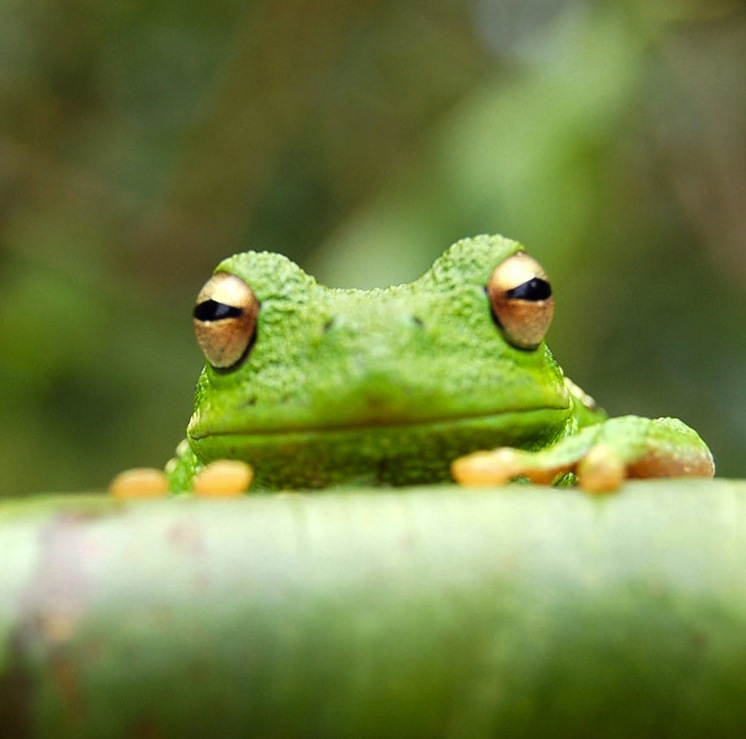
\includegraphics[width=\hsize]{frog}
% \caption{A half-columnwidth image using wrapfigure, to be used sparingly. Note that using a wrapfigure before a sectional heading, near other floats or page boundaries is not recommended, as it may cause interesting layout issues. Use the optional argument to wrapfigure to control how many lines of text should be set half-width alongside it.}
% \label{fig:halfwidth}
% \end{wrapfigure}


% \begin{figure}
% \begin{fullwidth}
% 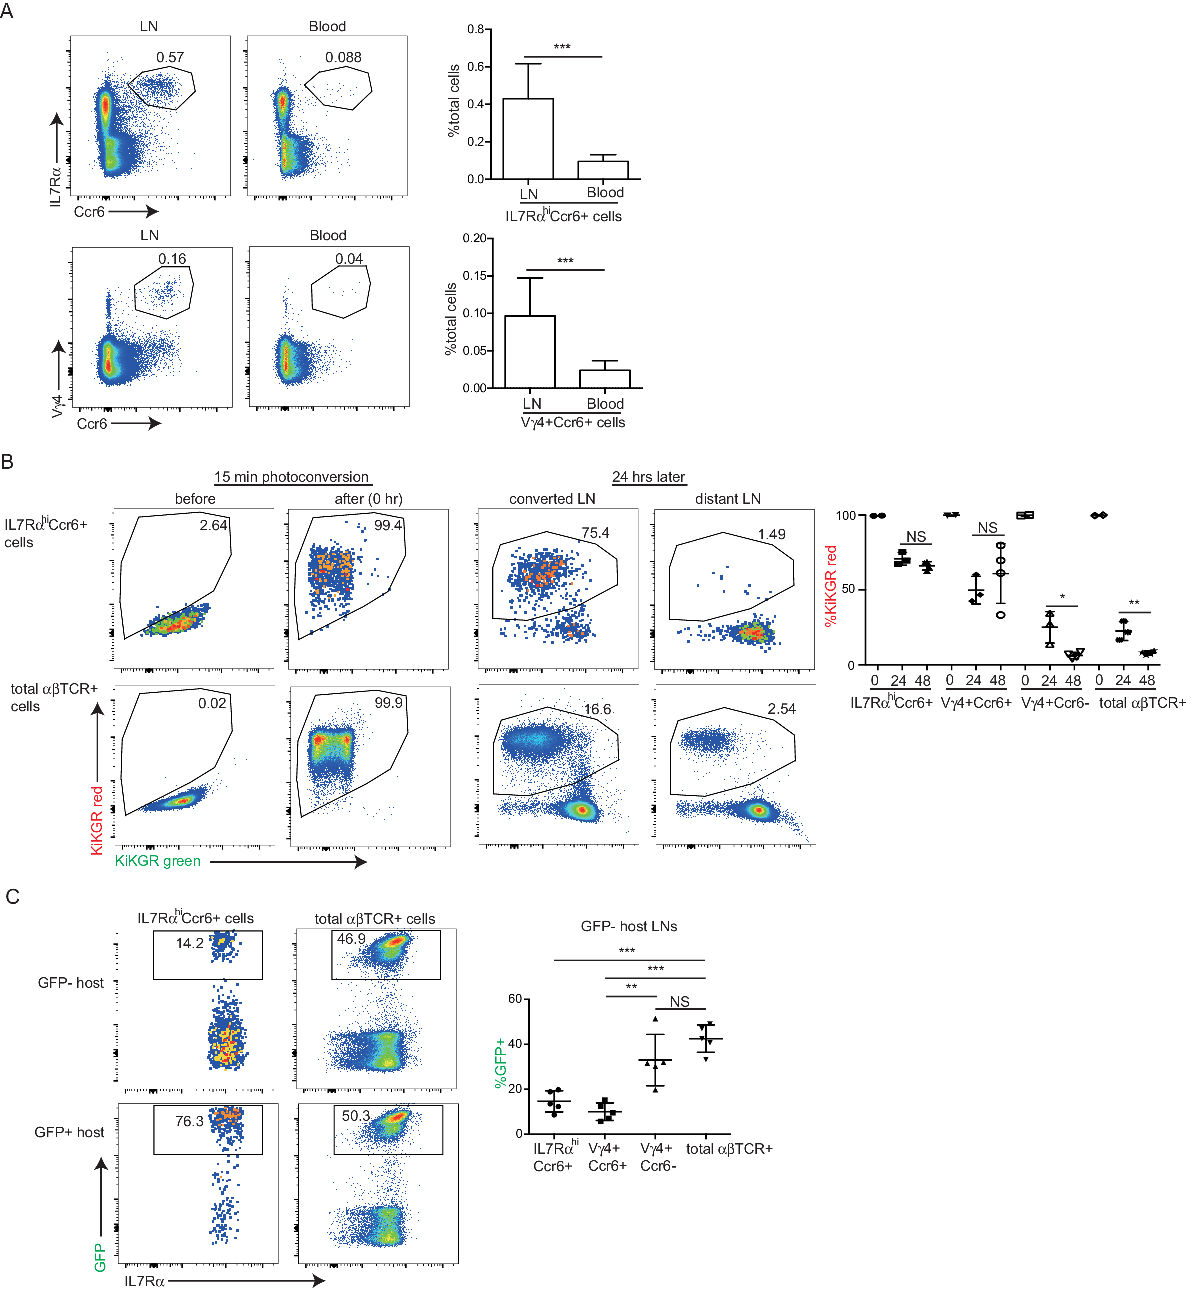
\includegraphics[width=0.95\linewidth]{elife-18156-fig2}
% \caption{A very wide figure that takes up the entire page, including the gutter space.}
% \label{fig:fullwidth}
% \figsupp{There is no limit on the number of Figure Supplements for any one primary figure. Each figure supplement should be clearly labelled, Figure 1--Figure Supplement 1, Figure 1--Figure Supplement 2, Figure 2--Figure Supplement 1 and so on, and have a short title (and optional legend). Figure Supplements should be referred to in the legend of the associated primary figure, and should also be listed at the end of the article text file.}{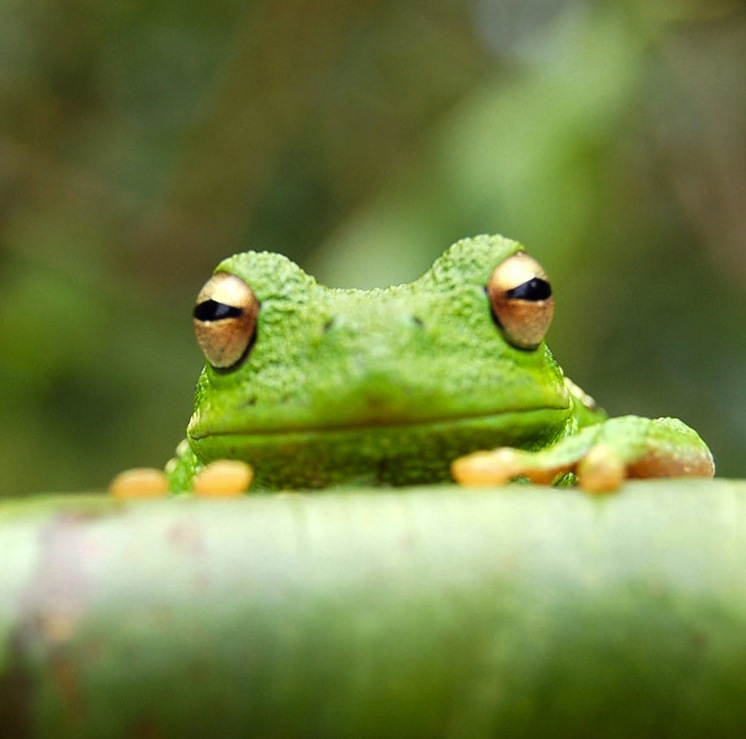
\includegraphics[width=5cm]{frog}}
% \end{fullwidth}
% \end{figure}


% \figsupp[Shorter caption for main text.]{This is a supplementary figure's full caption, which will be used at the end of the manuscript.}{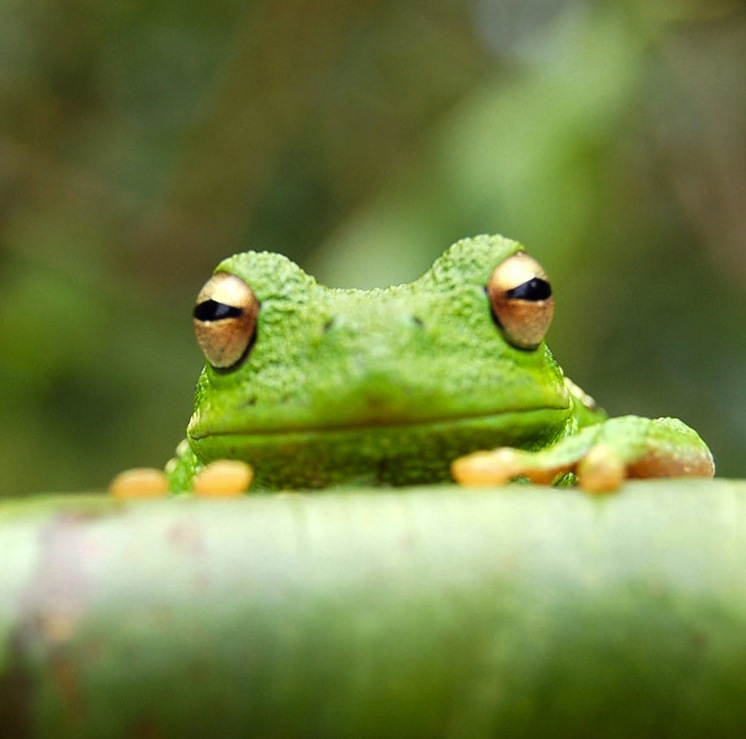
\includegraphics[width=6cm]{frog}}\label{figsupp:sf1}
% \figsupp{This is another supplementary figure.}{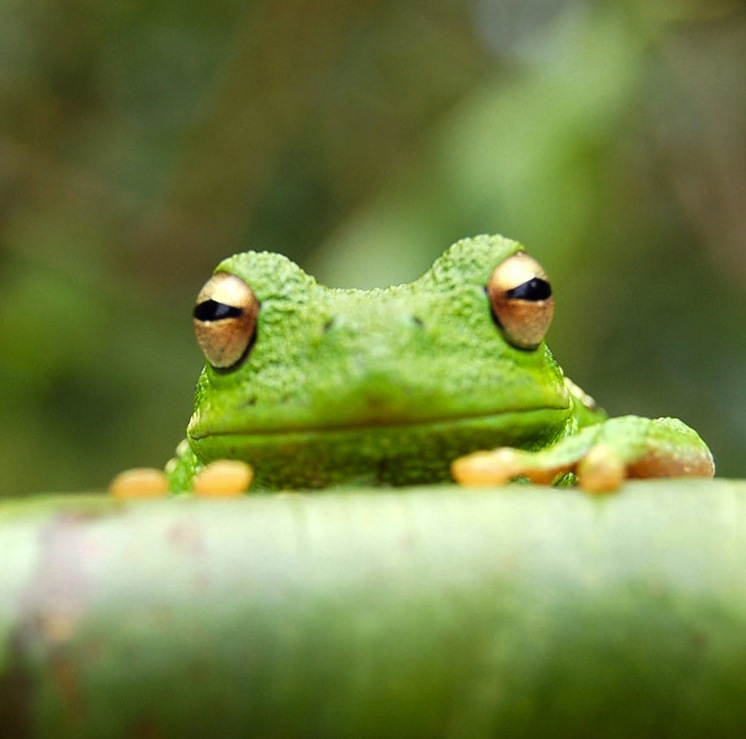
\includegraphics[width=6cm]{frog}}
% \videosupp{This is a description of a video supplement.}\label{videosupp:sv1}
% \figdata{This is a description of a data source.}\label{figdata:first}
% \figdata{This is another description of a data source.}\label{figdata:second}






% \section{Acknowledgments}

% Additional information can be given in the template, such as to not include funder information in the acknowledgments section.

% \nocite{*} % This command displays all refs in the bib file. PLEASE DELETE IT BEFORE YOU SUBMIT YOUR MANUSCRIPT!
\bibliography{library.bib}

%%%%%%%%%%%%%%%%%%%%%%%%%%%%%%%%%%%%%%%%%%%%%%%%%%%%%%%%%%%%
\end{document}
